\documentclass[letterpaper,12pt]{article}
\usepackage[utf8]{inputenc}

\usepackage{rotating}
\usepackage[top=1in, bottom=1in, left=1in, right=1in]{geometry}
\usepackage{graphicx}
\usepackage[numbers,square,sort&compress]{natbib}
\usepackage{setspace}
\usepackage[cdot,mediumqspace,]{SIunits}
\usepackage{hyperref}
\usepackage{mathtools}
\usepackage{url}
\usepackage{authblk}
\usepackage{placeins}
\usepackage{float}

\onehalfspacing
\title{Spectroscopy of Stars and CCD Properties }
\author{Anita Bahmanyar \qquad Ayushi Singh \qquad Carly Berard \\Department of Astronomy and Astrophysics, University of Toronto}
\affil{\small {anita.bahmanyar@mail.utoronto.ca}}
%\affil{\small {anita.bahmanyar@mail.utoronto.ca}}
\date{November 4, 2013}

\usepackage{graphicx}

\begin{document}

\maketitle

\begin{abstract}
\label{abstract}
In this lab, we learnt the method of spectroscopy, which is a very useful technique in astronomy. We used USB 2000 spectrometer to collect data from different sources including the Sun, Neon lamp, the Fluorescent lamp and some stellar objects such as Vega, Erif and Albeiro binary system. In this report, you will see the method of scaling between wavelength and pixel using Neon light, and some methods to investigate the noise properties of the detector such as gain, read-noise and saturation level. You will also see the spectrum of some stellar objects and how we can extract information such as temperature and the elements present in the stars using only their spectrum and then we compare their spectrum with blackbody spectrum.
\end{abstract}

%Introduction
\section{Introduction}
\label{sec:introduction}
Spectroscopy is a very powerful method in astronomy, since it enables us to measure both chemical and physical properties of celestial objects such as temperature, chemical elements present in the source, pressure and etc. The spectrometer that we used in this lab consisted of a 1-dimensional CCD detector. The CCD detector is made of Silicon and works based on photoelectric effect.  The charges in CCD are converted to voltage by the amplifier and then the voltage is converted to digital number, which is proportional to intensity of light, to make the image. CCDs do not have 100 percent efficiency, and there is always noise, including thermal noise. Therefore, it is common to keep the CCDs cool. The CCD we used for taking spectrum from objects using the campus telescope, was at -11 degrees celsius.

%Experimental Procedure
\section{Experimental Procedure}
\label{sec:experimental procedure}
\subsection{Equipment}
In order to collect data from different sources, we used USB 2000 spectrometer from Ocean Optics, which is an optical instrument based on diffraction grating to disperse light and a one-dimensional CCD array with 2048 pixels. Therefore, the data consisted of 2048 pixels as the first column and the intensity of the light coming in as the second column. This instrument achieves a spectral resolution of about 0.6 nm between wavelengths 370 to 700 nm.[1]

\subsection{Data Collcetion}
To start collecting data, we used SpectraSuite software installed on the computer connected to the spectrometer. We collected 100 sets of data from different sources including the Sun, Neon lamp, fluorescent lamp that was the lamp on the ceiling of the lab and the desk lamp. We collected the data from these sources more than once, each with different integration time, so that we were able to see the effect of integration time on the shape of the spectrum of the sources.
Then, we put the cap of the spectrometer sensor on top of it in order to prevent light coming in, and we got spectrum with the same time exposures. These data sets are called the dark signals of the sources. 



\section{Analysis}
\label{analysis}
\subsection{Wavelength Calibration}
We calibrated the wavelength using the data sets from Neon Lamp with 6 scans (to increase the accuracy), since we do not trust the manufacturer's wavelength calibration and it would be a good experience to do so. Wavelength calibration is the process of mapping the pixel number and wavelength versus each other. We did this by finding the centroids of the plot (the centre of the pixels we determined to be peaks), so we could find the local maximum points. These local maximum points are the bright emission lines in the lamp. Figure 1 and 2 show the spectrum of the Sun and the Neon lamp respectively. 


\FloatBarrier
\begin{figure}
\centering
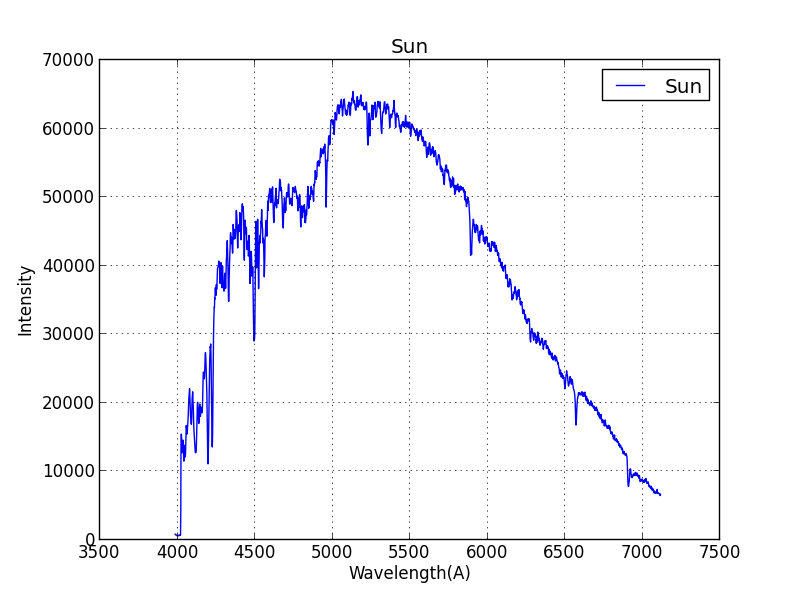
\includegraphics[scale=0.5]{sun_wavelength.png}
\caption{Sun Spectrum}
This figure shows the spectrum of the Sun with 15 s integration time and it is dark subtracted.
\end{figure}
\FloatBarrier


\FloatBarrier
\begin{figure}
\centering
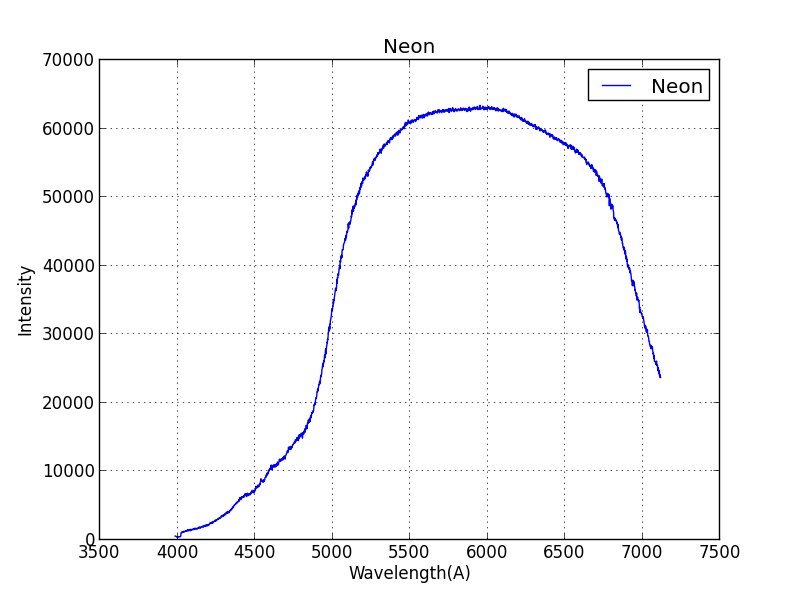
\includegraphics[scale=0.5]{neon_wavelength.png}
\caption{Neon Spectrum}
This figure shows the spectrum of the Neon Lamp with 100 ms integration time and it is dark subtracted.
\end{figure}
\FloatBarrier


We then plotted the wavelength vs. pixel number to find the relation between them. Then, we used the method given in the lab handout to find the fitting line. Below is the relation between pixel and wavelength for the Neon lamp that we obtained, using the fit line, and we used it to calculate all the other wavelengths for other pixels of the spectrometer. We also did the same procedure for the spectrometer on the telescope, with the Neon lamp there.Table 1 shows the pixel numbers corresponding to its wavelength. Using the numbers given in table 1 and plotting it as in Figure 3, we get the relation between wavelength and pixel, to be:
\newline
\begin{math}
y=1.529993 x + 3984.520672
\end{math}


Where y corresponds to wavelength and x corresponds to pixel numbers.


%\FloatBarrier
\begin{figure}[b!]
\centering
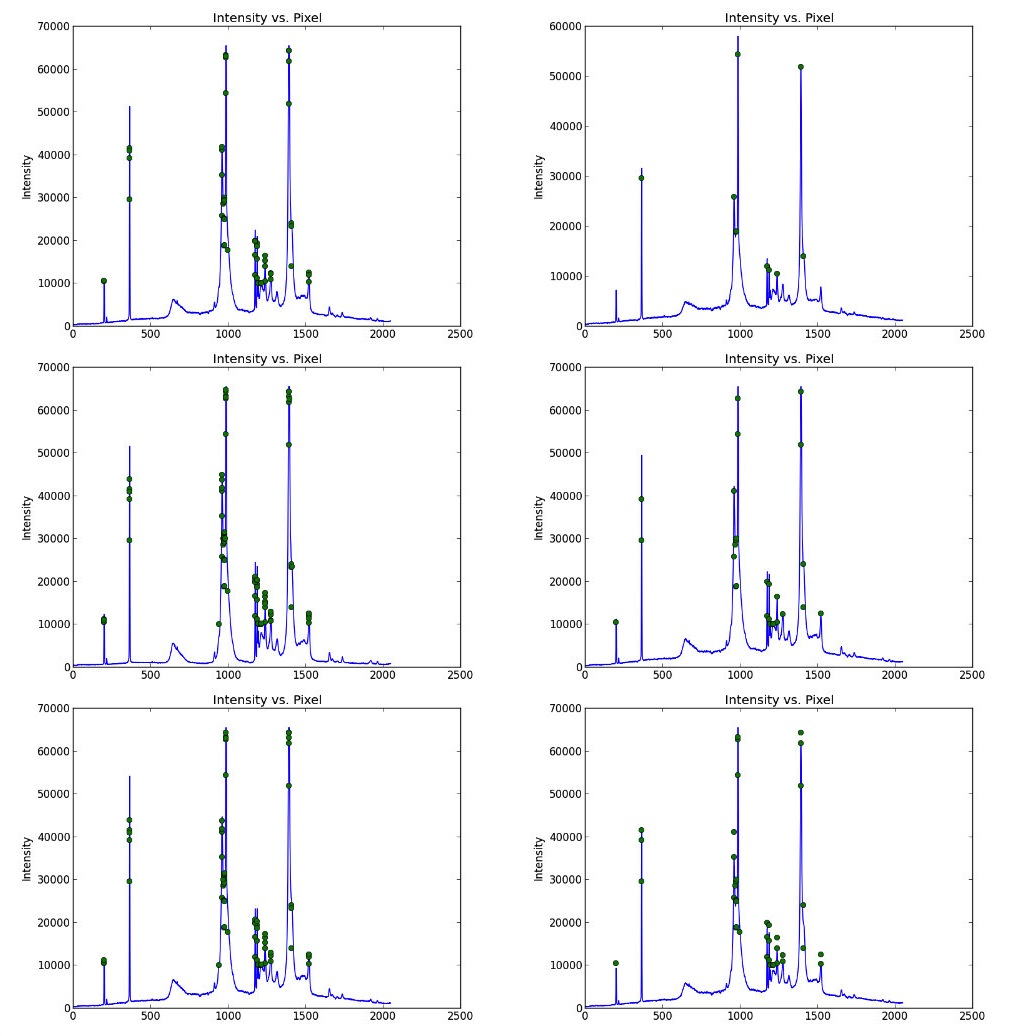
\includegraphics[scale=0.3]{mapping1.jpg}
\caption{Wavelength calibration}
The green dots show the local maximum points on the plot.s
\end{figure}
%\FloatBarrier



%\FloatBarrier
\begin{figure}[t!]
\centering
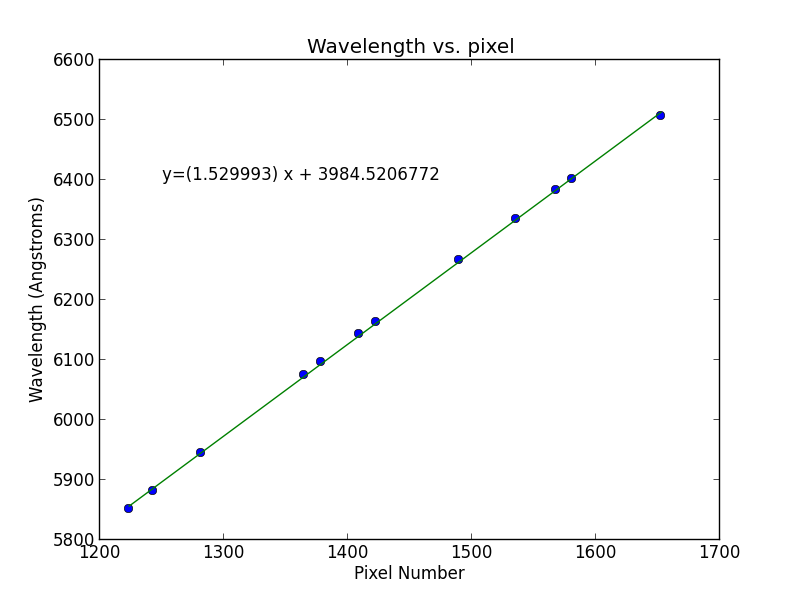
\includegraphics[scale=0.5]{linear_fit_first.png}
\caption{Linear Fit}
This figure shows the wavelength vs. pixel number plot, and also the linear fit for these values. As it is shown in the figure, there is a very good linear relation between wavelength and pixel number and enables us to get a linear mapping equation between wavelength and pixel number.
\end{figure}
%\FloatBarrier
After finding the centroids and plotting the results, we also plotted the residuals between the fit line and the actual data. As seen in Figure 3, linear residual is in range [-6,6].



\FloatBarrier
\begin{table}
\caption{Wavelength vs pixel number Residuals} % title of Table
\centering % used for centering table
\begin{tabular}{c c} % centered columns (4 columns)
\hline\hline %inserts double horizontal lines
Centroids(Pixel Numbers) & Corresponding Wavelength\\ [0.5ex] % inserts table
%heading
\hline % inserts single horizontal line
1223.5 & 5852.49\\ % inserting body of the table
1242.5 & 5881.89 \\
1281.5 & 5944.83 \\
1364.5 & 6074.34 \\
1378.5 & 6096.16 \\ 
1408.5 & 6143.06 \\ 
1422.5 & 6163.59 \\
1489.5 & 6266.49 \\
1535.5 & 6334.43 \\
1567.5 & 6382.99 \\
1580.5 & 6402.25 \\
1652.5 & 6505.53\\ [1ex] % [1ex] adds vertical space
\hline %inserts single line
\end{tabular}
\label{table:nonlin} % is used to refer this table in the text
\end{table}
\FloatBarrier


%\FloatBarrier
\begin{figure}[t!]
\centering
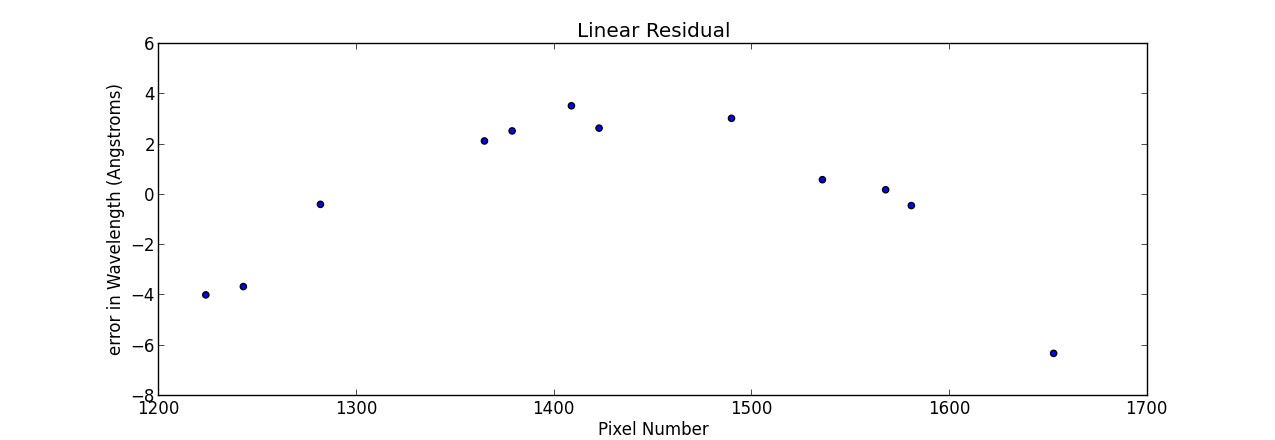
\includegraphics[scale=0.5]{linear_residual.png}
\caption{Linear fit Residuals}
This figure shows the residual between our data and the fitting line. It is in range [-6,6].
\end{figure}
%\FloatBarrier


\subsection{Gain, Read-Noise and Saturation Level}
Gain is defined as the number of electrons needed to produce 1 DN (Digital Number).  Read noise is the Electronic noise present in the CCD and creates unwanted signals. Gain and Read Noise were calculated by fitting a linear line to the variance vs. mean of the data. Below is the relation between variance and mean:
\begin{equation}
S_{adu}^{2}=S_{0}^{2}+kx_{adu}
\end{equation}
Where \begin{math} S_{adu}^2  \end{math}is the variance, \begin{math} S_{0} \end{math} is the read noise, k is the gain and \begin{math}x \end{math} is the mean pixel value. Therefore, by fitting a line to the data, we found the read noise to be -3380 (where the read noise is the square root of \begin{math} S_{0} \end{math}) and the gain to be 1.44. However, as we can see, the read noise value is negative which does not make any sense and the reason is that the fitted line has its intercept with y-axis in the negative part of the y-axis, whereas the data points have their intercept with y-axis in the positive part. Therefore, we needed to fit a non-linear curve and take its intercept as the read noise value. This turned out to be 1207.
There is a limit to the number of photons the spectrometer can detect. So, when the number of electrons entering the CCD exceeds the capacity of the each pixel, we say it is saturated. The saturation level of the spectrometer is independent of the source that we take the spectrum of. It only depends on the properties of the CCD pixels. In order to find out what the saturation level of the CCD we used in the lab as, we took multiple scans of higher exposure time (1 s) to saturate the pixels with photoelectrons. Then, we loaded the files into a python script and found the maximum intensity for each of the data sets, and this happened to be at 65535.0 data numbers. (\begin{math} (2^{16}-1 )\end{math}, since the analog to digital convert is 16-bit)
After this number, the photons do not increase the intensity of the light anymore and it results in spilling of excess electrons into the adjoining pixels. Figure 6 shows the saturated spectrum of the CCD.


\FloatBarrier
\begin{table}
\caption{Wavelength vs pixel number Residuals} % title of Table
\centering % used for centering table
\begin{tabular}{c c c} % centered columns (4 columns)
\hline%inserts double horizontal lines
Gain & Read-Noise & Saturation Level\\ [0.5ex] % inserts table
%heading
1.44 & 1207 & 65535\\ [1ex] % [1ex] adds vertical space
\hline %inserts single line
\end{tabular}
\label{table:nonlin} % is used to refer this table in the text
\end{table}
\FloatBarrier


\begin{figure}[t!]
\centering
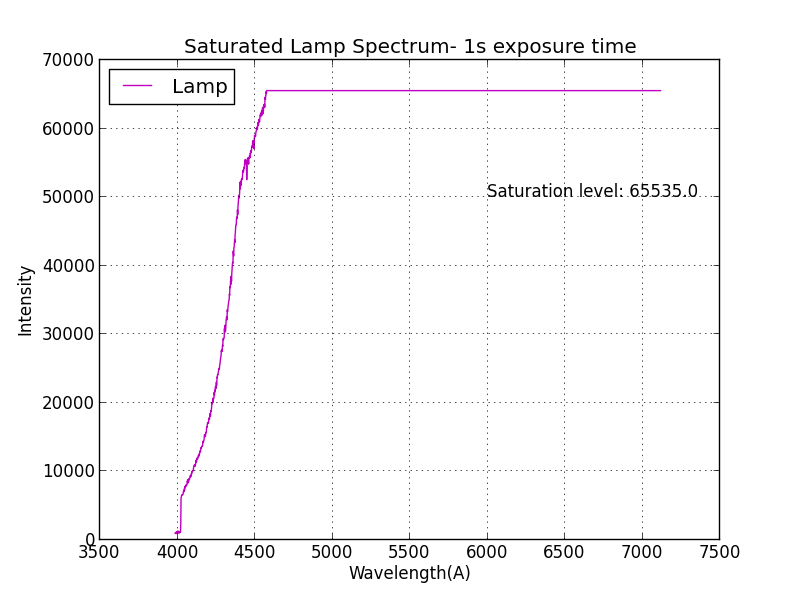
\includegraphics[scale=0.5]{saturation_level.png}
\caption{Saturation Level of the CCD }
This figure shows the saturation level of the CCD, that is obtained by exposing the sensor for 1 s.
\end{figure}



\subsection{Telescope Data}
We collected data from telescope in two different nights, so we have different sources. We took the spectrum of Vega with three different integration times, Erif with two different integration times, Albeiro that is a binary star system and Scheat. We also collected the dark frames for each of these sets. We then did the same method for mapping between wavelength and pixels to get the wavelength scale, since the data from the telescope was also in pixels and intensity. This time we used the neon lamp in the telescope room. So we got the fitting line to be \begin{math} y= 1.44 x +1207 \end{math}.
We had to flip the data we got from the telescope, since it was backwards. At first, when we were trying to map the wavelength and pixels, the numbers were really off from the theoretical values, and when we flipped the data we saw a good relationship between the data we got and the theoretical values.

\section{Discussion}
\label{discussion}
First of all, we should apply the corrections to the spectrum of the stars taken with the telescope. We should use equations 2, 3 and 4 in order to correct for the wavelength of the peak, since without correction, peak of all of the spectrums are almost at the same wavelength, which is not correct. After applying equation 2, 3 and 4 to the data and then plotting, we got the blue shifted and red shifted spectrum of the stars and therefore, the wavelength of the maximum intensity are correct.
\begin{equation}
p_{i}=\frac{R_{i}-D_{i}}{L_{i}-D_{i}}B(v,T)
\end{equation}

\begin{equation}
B(v,T)=\frac{2hv^{3}}{c^{2} e^{hv/kT}-1}
\end{equation}

\begin{equation} v_{i}=\frac{c}{\lambda_{i}} \end{equation}

Where \begin{math}  B(v,T)  \end{math} is the Planck's function. 
\begin{figure}[b!]
\centering
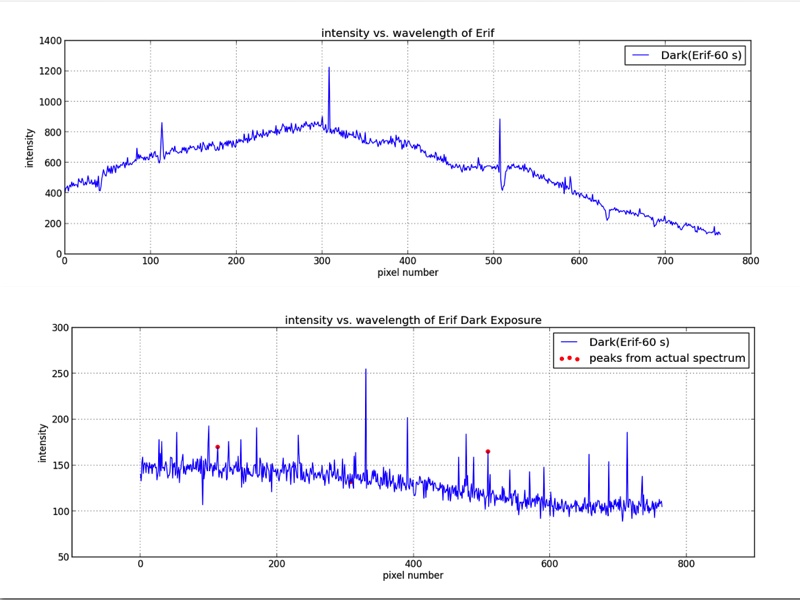
\includegraphics[scale=1.6]{erif_comparison.jpg}
\caption{Spectrum of Erif}
This figure shows that the peaks at pixels 113 and 509 are from the noise, since they also exist in the dark exposure; however, the peak from pixel number 308 is not from the noise in the CCD and it might be the atmospheric emission line.
\end{figure}

From the spectrum of the stars, we are able to get the temperature. Since the spectrum we plotted is in intensity vs. wavelength and by Wien displacement law, which is given in equation 4 we can get the temperature of the blackbody:

\begin{equation}
T_{blackbody}=0.002928/\lambda_{max}
\end{equation}
Where \begin{math} \lambda_{max} \end{math} is the wavelength of the maximum intensity.
We got the temperature for Vega to be approximately ~6400 K.
We can see some Hydrogen alpha and Hydrogen beta absorption lines at 656 nm and 486 nm present in Vega spectrum respectively.
Comparing the two spectrum taken from Albeiro, we can see that the two spectrums are completely different and the reason is that Albeiro is a binary star system and each of the spectrums are for one of the stars. We can see emission lines from one of these spectrum and it is probably the noise(and not emission line from accretion of gas), since it is only peaked at one sharp point unlike the wide absorption lines. Moreover, by looking at its dark counts, we can confirm it is due to noise. This occurs at pixel numbers 113, 308 and 509. These are shown in figure 4. However, the very thin and sharp peak at pixel number 308 does is not due to the noise in dark exposure, since it is not a peak point in dark exposures as seen in figure 6, so it might be the emission line from Earth's atmosphere.

\begin{figure}[H]
\centering
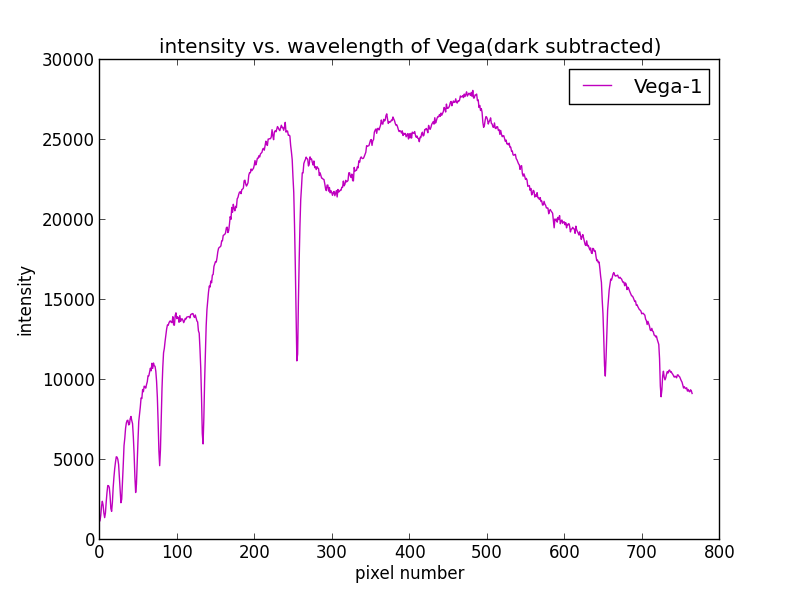
\includegraphics[scale=0.6]{vega-01-dark_subtracted.png}
\caption{Spectrum of Vega}
This figure shows the spectrum of Vega with 15 s integration time. These absorption lines are mostly from Hydrogen, including Hydrogen alpha and Hydrogen Beta. This is the dark subtracted data.
\end{figure}

We can also talk about temperature of these stars. Vega peaks at about ~450 nm, which corresponds to ~6400K using equation 3. This is almost the temperature of the Sun which is a G type star; however, from theoretical data we know Vega is an A type star and has temperature of approximately ~9300 K. One hypothesis we came up with was that maybe Vega does not have its peak in visible wavelength and the peak wavelength we are considering is only the visible peak, therefore the temperature from theoretical data might be considering the maximum intensity of Vega in all of the wavelengths. Figure 8 shows the spectrum of Vega with 15 s exposure time.

We can also determine some properties of the CCD such as read-noise, gain and saturation level. We got the gain value to be 1.44 . As it can be seen in figure 9, the variance vs. mean is not linear over the whole range, so in order to get a linear fit, we cut out parts from 500 to 900.



\begin{figure}[H]
\centering
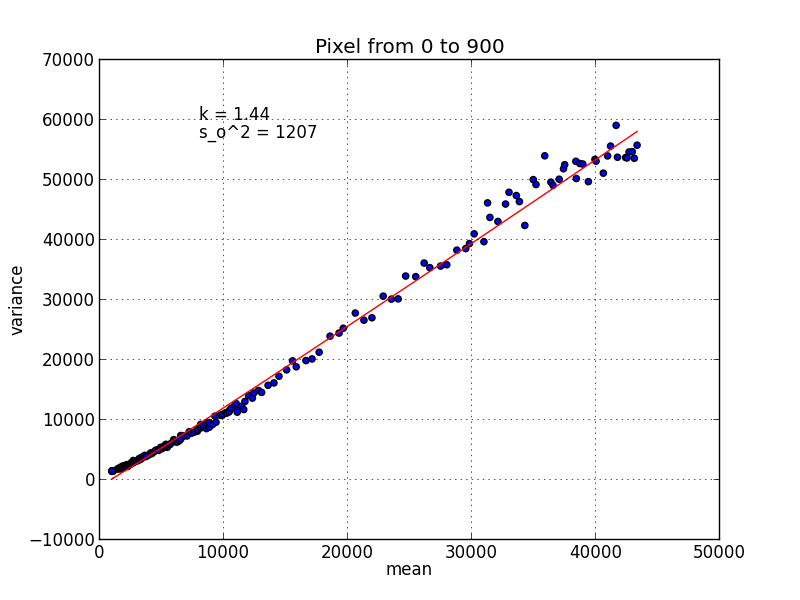
\includegraphics[scale=0.6]{noise3.png}
\caption{Read-Noise and Gain of CCD}
This figure shows the variance plotted vs. the mean of our data. By fitting  a line, we can determine the gain and read-noise values for the CCD we used using equation 1.
\end{figure}

\section{Conclusion}
\label{conclusion}
Through this lab, we learnt how to use spectrometer and CCD detector. Noise can have effect on our data and there are different types of noise that we have to consider, for instance read-noise and thermal noise. Therefore, we had to consider dark exposures in order to account for the thermal noise in the CCD. There was also error in the scaling method we used, since conversion between wavelength and pixel number is not perfect and the linear relation we got is not completely fitting the data.
CCD detectors are used in astronomical spectroscopy to gather information about distant objects. Spectroscopy enabled us to calculate temperature of stars and to figure out what elements are present in each of the sources.




\section{References}
\label{references}
[1]-Lab \# 2 Handout

\end{document}
